\chapter{[Por revisar] Metodología}
\label{chapter:metodologia}

\chapquote{Caer está permitido, levantarse es obligatorio.}{Proverbio ruso}

En primer lugar, se puede definir como metodología de desarrollo software al conjunto de técnicas, prácticas y métodos que se utilizan para diseñar e implementar un sistema basado en \textit{software}, con la finalidad de organizar de la mejor manera posible los equipos de trabajo involucrados en el desarrollo software \cite{santander_universidades_metodologias_2020}.

La elección de la metodología para un proyecto de desarrollo software depende de factores como el tamaño del equipo de desarrollo del proyecto, los requisitos del mismo y su posible cambio, las restricciones de tiempo... Asimismo, dicha elección impacta notablemente en ámbitos como la gestión de los recursos, la planificación de las actividades, la comunicación entre los miembros del equipo o a la evaluación de la calidad del producto.

\section{Metodologías de desarrollo del \textit{software} de Sistemas}

    Las metodologías para el desarrollo de software han sufrido una constante evolución desde su aparición en los años 60 del siglo pasado y presentan grandes diferencias entre sí. En esta sección serán introducidas algunas de las metodologías más relevantes, remitiendo al lector a las publicaciones citadas si desea profundizar en las mismas.

    \subsection{Metodologías Tradicionales}
    
        Estas metodologías se basan en una estructura lineal, donde se completan las fases del desarrollo en secuencia. El calificativo tradicional se debe a su creación en las primeras etapas de la Ingeniería del Software.
    
        \begin{itemize}
        \item Cascada: este modelo, según  \cite{sommerville_software_2011}, separa las actividades fundamentales tales como la especificación, desarrollo, validación y evolución, en una secuencia de fases: definición de requerimientos, diseño del sistema software, implementación y prueba de unidad, integración y pruebas del sistema y, por último, operación y mantenimiento. El desarrollo se lleva a cabo completando cada una de estas fases de forma secuencial, pudiendo regresar a cualquiera de las fases anteriores solo tras haber completado previamente la secuencia completa.
    
        Por otra parte, existen modificaciones de esta metodología, como \textit{cascada con retroalimentación}, que añaden la posibilidad de volver a la fase anterior de desarrollo en caso de identificarse problemas, sin necesidad de finalizar todas las etapas; como puede verse en la figura \ref{fig:metodologia:cascada_retroalimentada}.
    
        \begin{figure}[h]
            \centering
            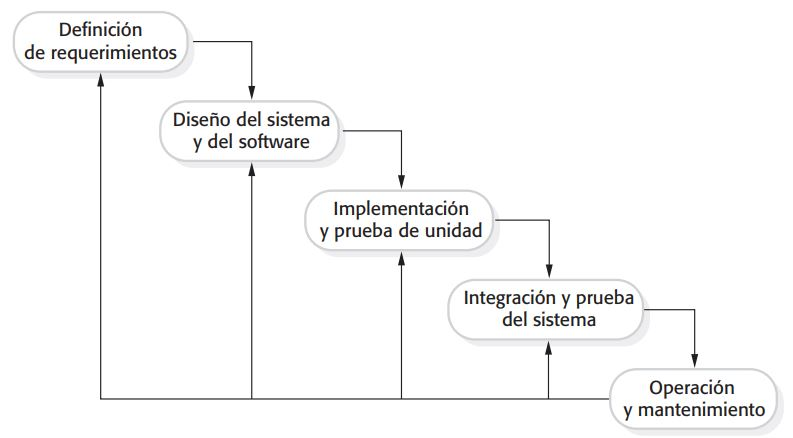
\includegraphics[width=0.66\textwidth]{figures/cascada retroalimentada.JPG}
            \caption[Modelo en cascada con retroalimentación, extraído de \cite{sommerville_software_2011}]{Modelo en cascada con retroalimentación.}
            \label{fig:metodologia:cascada_retroalimentada}
        \end{figure}
        
        \item Modelo en V: considerado como una variante de la metodología en cascada, se representan las acciones a seguir en una V, como se puede ver en la Figura \ref{fig:metodologia:modelo_v}. Según \cite{pressman_software_2005}, a medida que el equipo de software avanza hacia abajo desde el lado izquierdo de la V, los requerimientos básicos del problema mejoran hacia representaciones técnicas cada vez más detalladas del problema y de su solución. 
        
        Una vez que se ha generado el código, el equipo sube por el lado derecho de la V, y en esencia ejecuta una serie de pruebas (acciones para asegurar la calidad) que validan cada uno de los modelos creados cuando el equipo fue hacia abajo por el lado izquierdo donde se aprecia la relación entre las acciones para  el aseguramiento de la calidad y aquellas asociadas con la comunicación, modelado y construcción temprana. 
    
        \begin{figure}[h]
            \centering
            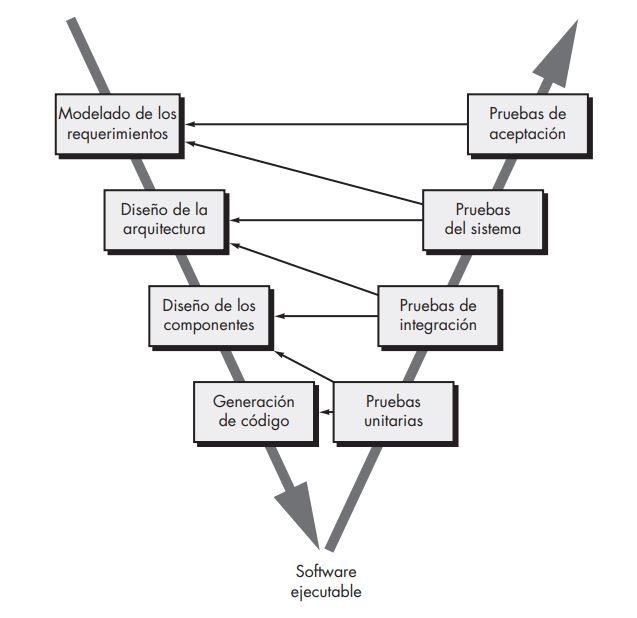
\includegraphics[width=0.5\textwidth]{figures/en v.JPG}
            \caption[Modelo en V, extraído de \cite{pressman_software_2005}]{Modelo en V.}
            \label{fig:metodologia:modelo_v}
        \end{figure}
    \end{itemize}

    \subsection{Metodologías Ágiles}

        Este conjunto de métodos deben su nombre al \textit{Manifiesto Ágil} \cite{varios_autores_manifiesto_2001}, donde se reivindica un enfoque que apueste por ``individuos e interacciones sobre procesos y herramientas, software funcionando sobre documentación extensiva, colaboración con el cliente sobre negociación contractual y respuesta ante el cambio sobre seguir un plan``. Algunas de las metodologías que implementan estos principios son:
    
        \begin{itemize}
            \item Scrum, si bien es previa al \textit{Manifiesto Ágil}, sus principios son congurentes con el manifiesto. En esta aproximación se utiliza un enfoque iterativo para el desarrollo, bajo el concepto de \textit{sprint}, tal y como se puede visualizar en la Figura \ref{fig:metodologia:scrum} . Un \textit{sprint} es una unidad de trabajo de duración fija (normalmente dos semanas) en la cual no se pueden introducir cambios, permitiendo cierta estabilidad a la vez que se abraza el cambio \cite{pressman_software_2005}. 
    
            \begin{figure}[h]
                \centering
                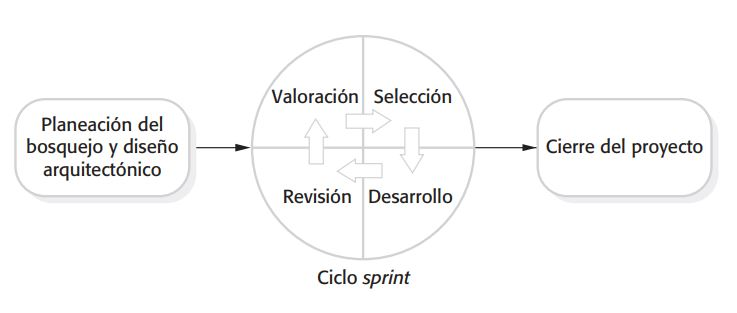
\includegraphics[width=0.66\textwidth]{figures/scrum.JPG}
                \caption[El proceso de Scrum, extraído de \cite{sommerville_software_2011}]{El proceso de Scrum}
                \label{fig:metodologia:scrum}
            \end{figure}
            
            Asimismo, en esta unidad de tiempo se incorporan una serie de reuniones o ceremonias, tales la reunión diaria o \textit{daily} ,en la que en 15 minutos cada integrante del equipo expresa qué ha hecho desde la reunión anterior, sus planes de cara a la siguiente y los obstáculos que está encontrando; la \textit{Sprint Planning}, en la que el equipo de desarrollo decide las tareas a realizar en el siguiente sprint, o la \textit{Sprint Retrospective}, donde se analiza la ejecución del sprint anterior para plantear posibles mejoras. 
    
            Por otra parte, se definen roles en el equipo tales como \textit{Scrum Master}, el cual se encarga de la comunicación con otros equipos y clientes, modera las reuniones y registra las decisiones entre otras cuestiones, o el \textit{Product Owner}, siendo el responsable del proyecto en cuanto al desarrollo, mantenimiento y priorización de las tareas \cite{valtx_metodologias_2023}.
    
            \item Kanban es una metodología ágil creada por Toyota, la cual tiene como elemento diferenciador el uso de tarjetas visuales (kanban en japonés) \cite{pzt_metodologias_nodate}, representadas en forma de un tablero donde se refleja el flujo de los procesos en un trabajo designado, permitiendo a cada responsable mover sus tareas libremente según los avances. Ese flujo de trabajo puede ser algo tan sencillo como ``Por hacer``, ``En curso`` y ``Terminado`` \cite{atlassian_que_nodate-1}, como se puede ver en la figura \ref{fig:metodologia:kanban}.
    
            \begin{figure}[h]
                \centering
                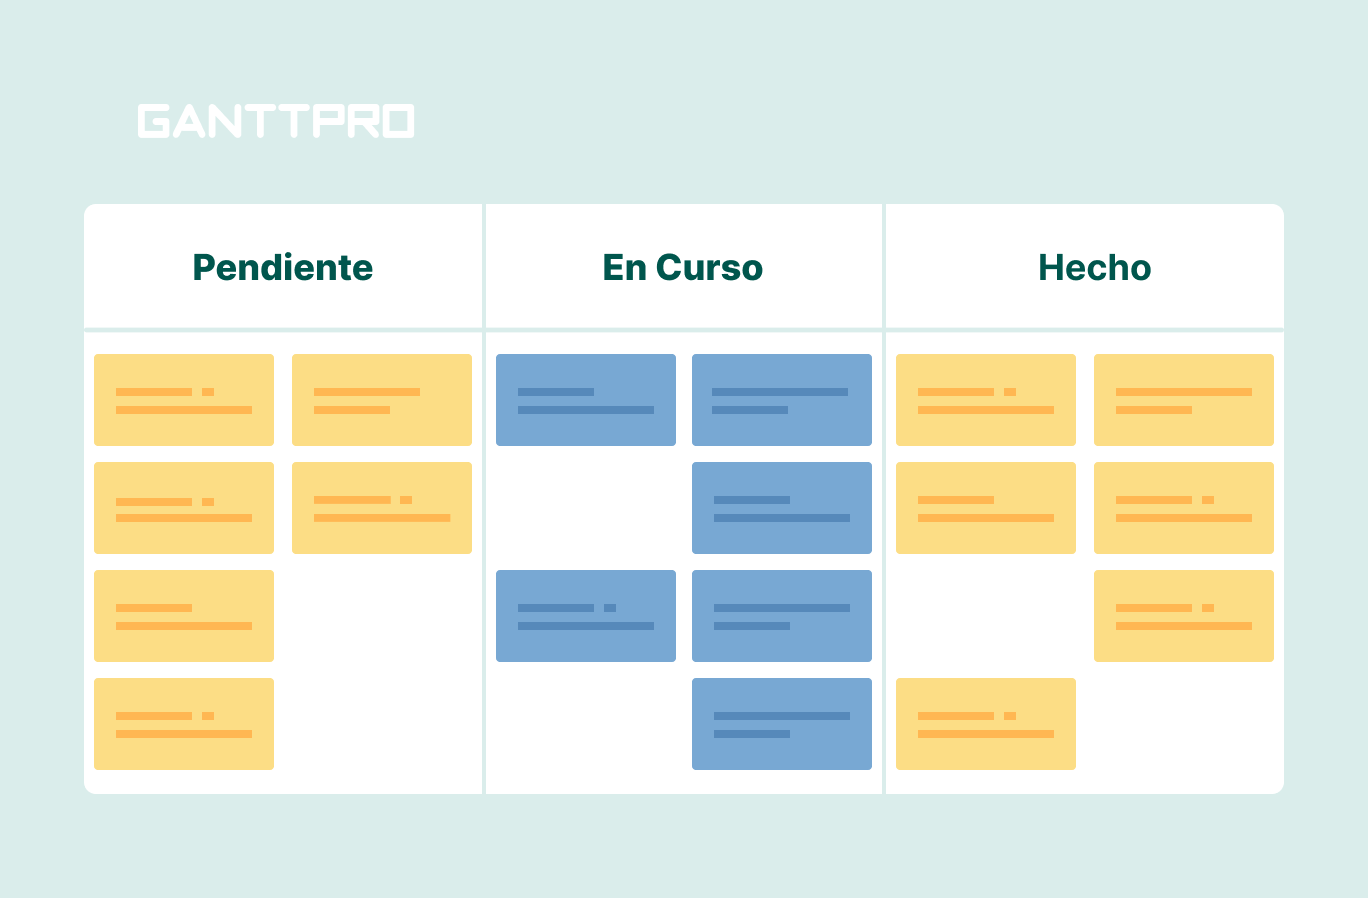
\includegraphics[width=0.66\textwidth]{figures/kanban.png}
                \caption[Tablero Kanban, extraído de \cite{stsepanets_metodo_2024}]{Tablero Kanban}
                \label{fig:metodologia:kanban}
            \end{figure}
            
    
            Según \cite{valtx_metodologias_2023}, algunos de sus principios son: 
    
            \begin{enumerate}
                \item Visualizar lo que hace. La visualización por parte de todos los responsables del proyecto en el flujo de las tareas permite mantenerse atentos sobre el desarrollo del proyecto.
                \item Limitar la cantidad de trabajo en proceso. El establecimiento de metas alcanzables permite al grupo un equilibrio en el flujo del trabajo y previene el exceso de procesos centralizados en pocos responsables.
                \item Realizar seguimiento del tiempo. El manejo del tiempo de forma organizada permite obtener resultados precisos en el proyecto.
                \item Lectura fácil de indicadores visuales. La visualización de los tipos de trabajo, prioridades, fechas y demás detalles empodera al equipo en el desarrollo de soluciones ajustadas a la realidad.
            \end{enumerate}
            
        \end{itemize}

\section{Metodología de desarrollo seleccionada}

    Para el desarrollo de este proyecto se ha elegido la metodología \textbf{en cascada con retroalimentación}, justificándose dicha elección con las siguientes razones:
    
    \begin{itemize}
        \item Equipo reducido: el equipo de desarrollo de este proyecto se ha compuesto únicamente por el autor, con la supervisión de sus dos directoras. Como se describió anteriormente, metodologías como Scrum definen una serie de roles claramente diferenciados; por lo que no se adaptan a un equipo tan reducido.
        \item Estabilidad de los requisitos: los requisitos que fundamentan este proyecto son definidos claramente desde el inicio, siendo poco propensos a ser modificados durante la ejecución del mismo. 
        \item Definición clara y sencilla de las fases: se busca una metodología que permita trabajar eficientemente, con la menor sobrecarga posible mientras se garantice la calidad. Al asumirse un cambio inexistente o relativamente pequeño, se puede contemplar el uso de metodologías tradicionales en lugar de las ágiles, al no necesitarse la sobrecarga de roles y ceremonias. 
        \item Retroalimentación periódica: si bien no se contemplan cambios significativos durante el desarrollo del proyecto, se desea cierta flexibilidad que permita descubrir y corregir errores de forma temprana. Metodologías tradicionales, como en cascada sin retroalimentación, muestran un enfoque muy rígido para la identificación y resolución de problemas durante el transcurso del proyecto.
    \end{itemize}